%% IEEE Conference şablonu — Kocaeli Haber Haritası Projesi Raporu
%% Derleme: pdflatex (2 kez) + bibtex (isteğe bağlı)
%%
%% Özet: \section*{Özet} ile Giriş/Yöntem başlığı stilinde; gövde düz (kalın değil).
%%
%% Fotoğraf: dosyayı rapor/ klasörüne koyun; aşağıdaki FIG_TEAM yorumunu okuyun.
%% Mimari şekil: kaynak rapor/mermaid_mimari.mmd — PNG/PDF üretmek için (rapor/ içindeyken):
%%   npx -y @mermaid-js/mermaid-cli -i mermaid_mimari.mmd -o resim/mimari_mermaid.png -b white
\documentclass[conference,a4paper]{IEEEtran}
\IEEEoverridecommandlockouts

\usepackage[T1]{fontenc}
\usepackage[utf8]{inputenc}
\usepackage{cite}
\usepackage{amsmath,amssymb}
\usepackage{graphicx}
\usepackage{textcomp}
\usepackage{float}
\usepackage{xcolor}
\usepackage{url}
\usepackage{booktabs}
\usepackage{tikz}
\usetikzlibrary{positioning, shapes.geometric, arrows.meta, fit, backgrounds, calc}

%% Görseller: .tex ile aynı klasör veya rapor/resim/ altı
\graphicspath{{./}{./resim/}}

\hyphenation{Kocaeli MongoDB Flask Beautiful-Soup}

\begin{document}

\title{%
  {\large\bfseries YazLab~2}\\[0.55em]%
  Kocaeli Bölgesi Yerel Haberlerinin Web Kazıma, Sınıflandırma ve Coğrafi Görselleştirilmesi%
}

\author{
\IEEEauthorblockN{Enes ÜLKÜ}
\IEEEauthorblockA{Öğrenci No: 230202083}
\and
\IEEEauthorblockN{Yunus Emre AYIKER}
\IEEEauthorblockA{Öğrenci No: 230202082}
}

\maketitle

% IEEE abstract ortamı yerine: başlık Giriş/Yöntem ile aynı \section* stili; metin kalın/italik değil.
\section*{Özet}
{\normalfont\normalsize\mdseries\upshape
Bu çalışmada Kocaeli ili yerel basınından çoklu kaynaklı haberlerin otomatik toplanması, metin ön işleme ve kural tabanlı sınıflandırma ile haritalanması sunulmaktadır. Sistem; Python tabanlı web kazıyıcılar, MongoDB veri tabanı, çok dilli cümle gömme modeli ile anlamsal tekrar tespiti, Google Geocoding API ile konum üretimi ve harita üzerinde etkileşimli bir arayüz içermektedir. Özet üretimi, başlık--cümle benzerliğine dayalı seçici (extractive) yöntemle iyileştirilmiştir. Bulgular, kural tabanlı sınıflandırmanın bağlam cezaları ve anahtar kelime ağırlıkları ile iyileştirilebildiğini; ancak sitelerin erişim politikalarının (ör.\ Cloudflare) kazıma kapsamını doğrudan etkilediğini göstermektedir.
\par}

\begin{IEEEkeywords}
web kazıma, haber sınıflandırması, coğrafi kodlama, MongoDB, harita görselleştirme, anlamsal benzerlik
\end{IEEEkeywords}

\section{Giriş}
Yerel haber siteleri, kentsel olaylar (trafik, güvenlik, altyapı, kültür) için zamanında bilgi sağlar; fakat kaynakların dağınıklığı, farklı CMS şablonları ve aynı olayı birden fazla sitede tekrarlayan içerikler, tek bir bakışta bölgesel durum farkındalığını zorlaştırır. Kullanıcıların beş farklı siteyi tek tek gezmesi hem zaman kaybıdır hem de olay türüne göre hızlı filtreleme imkânı sunmaz. Bu proje, belirli Kocaeli kaynaklarından haberlerin otomatik toplanması, metin ön işleme, olay türüne göre etiketlenmesi, mümkün olduğunda ilçe veya adres düzeyinde konum çıkarımı ve harita üzerinde etkileşimli sunulması hedefiyle tasarlanmıştır.

Sistem, ders kapsamında uçtan uca bir veri mühendisliği örneği olarak konumlandırılmıştır: ham web sayfasından başlayıp yapılandırılmış kayıt üretmek, bu kayıtları veri tabanında saklamak ve REST üzerinden harita istemcisine aktarmak zincirinin tamamı uygulanmıştır. Böylece yalnızca ``kazıma'' değil, kalite kontrol (tekrar, sınıf tutarlılığı) ve görselleştirme katmanları da raporun odağındadır.

Çalışmanın katkıları şunlardır: (i) çok kaynaklı boru hattı mimarisi ve kaynak başına özelleştirilmiş seçiciler, (ii) gömme tabanlı anlamsal tekrar birleştirme, (iii) Google Geocoding ile önbellekli konum üretimi, (iv) Flask tabanlı API ve web istemcisinde filtreleme, detay paneli ve kaynak bazlı sayım göstergeleri. Aşağıdaki bölümlerde önce kavramsal çerçeve, ardından mimari ve yöntem ayrıntıları, son olarak sahadan gözlemler ve kısıtlar tartışılacaktır.

\section{Problem Tanımı ve Kapsam}
Girdi, seçilmiş yerel haber sitelerinin liste ve haber detay URL'leridir. Çıktı ise her haber için en azından başlık, kaynak adı, tarih, tam metin veya özü, birincil kategori, varsa koordinatlar ve haritada gösterim için uygun meta verilerdir. Kapsam dışı bırakılan durumlar şunlardır: abonelik duvarı arkasındaki içerik, kullanıcı oturumu gerektiren sayfalar ve projede açıkça tanımlanmamış yeni kategori türleri (bunlar ya reddedilir ya da genel skor eşiğine takılır).

\section{İlgili Çalışmalar ve Kavramlar}
Web kazıma, yapılandırılmış veriyi HTML/XML sayfalarından çıkarma sürecidir; pratikte DOM ağacı üzerinde CSS seçicileri veya kalıp eşleştirme ile çalışılır \cite{scraping}. Siteler yapı değiştirdiğinde kırılmaya açık olduğundan, kazıyıcıların modüler ve kaynak bazlı izole edilmesi bakım maliyetini düşürür.

Haber sınıflandırmasında hem kural tabanlı hem de öğrenmeli yöntemler kullanılır. Derin öğrenme tabanlı sınıflandırıcılar yüksek doğruluk verebilir; ancak etiketli veri, eğitim süresi ve açıklanabilirlik maliyeti vardır. Bu projede düşük gecikme ve şeffaf kararlar için anahtar kelime ağırlıklı skorlama tercih edilmiş; bağlam cezaları ve URL ipuçları ile yanlış pozitifler azaltılmıştır.

Tekrar eden veya çok benzer haberler, kelime örtüşmesi yerine anlamsal yakınlık ile daha güvenilir biçimde eşlenebilir; bunun için önceden eğitilmiş cümle gömme modelleri yaygın olarak kullanılır \cite{reimers2019}. Kosinüs benzerliği eşik üzerindeyse kayıtlar birleştirilerek tek harita işaretçisi altında çoklu kaynak gösterilebilir.

Adreslerin enlem/boylama dönüştürülmesi için ticari coğrafi kodlama hizmetleri endüstride standarttır. Aynı metin için tekrarlı sorguları önlemek üzere sonuçların veri tabanında önbelleklenmesi hem API kotasını korur hem de boru hattı süresini kısaltır \cite{googlegeo}.

\section{Sistem Mimarisi}
Şekil~\ref{fig:arch} ile uyumlu olacak şekilde sistem üç ana katmandan oluşur: veri toplama, sunucu tarafı işleme ve ön uç sunum. Katmanlar gevşek bağlıdır; API sözleşmesi sabit kaldığı sürece yeni bir kaynak kazıyıcısı veya ek bir filtre bileşeni eklenebilir.

\subsection{Veri Toplama Katmanı}
Her kaynak için ayrı kazıyıcı sınıfları, ortak bir taban sınıftan türetilir. Bu sayede ortak HTTP başlıkları, zaman aşımı, hata günlüğü ve isteğe bağlı yeniden deneme politikası tek yerde toplanır. Liste sayfalarından haber URL'leri toplanır; her URL için ayrıntı sayfasından başlık, mümkünse yayım tarihi ve gövde metni çıkarılır. Tarih alanları bazen göreli ifadeler (``dün'', ``bugün'') veya farklı yerel biçimler içerdiğinden, ayrıştırıcıların siteye özel ince ayarı gerekir.

Erişim engellerini hafifletmek için oturum çerezleri ve isteğe bağlı \texttt{cloudscraper} kullanımı desteklenir. Buna karşın tüm kaynakların her çalıştırmada aynı koşullarda erişilebilmesi garanti edilmez: bazı alan adları agresif WAF kuralları, bot skorlaması veya coğrafi kısıt uygulayabilir. Bu durumda sistem, hatayı günlükleyerek diğer kaynakların işlenmesine devam eder; kullanıcı arayüzünde kaynak bazlı sayımlar eksikliği görünür kılar.

\subsection{İşleme Boru Hattı}
Boru hattı aşamaları sırayla şunlardır: ham metin temizleme (HTML artığı, fazla boşluk, bazı kalıp ifadeler), kategori sınıflandırması, Kocaeli odaklı konum adayı çıkarımı, haber metni için gömme vektörü üretimi ve veri tabanındaki mevcut gömelerle tekrar karşılaştırması, gerekirse geocoding zinciri ve nihai kaydın yazılması. Çoklu iş parçacığı ile kaynaklar paralel taranır; tekrar tespiti ve yazma adımlarında tutarlılık için eşzamanlılık kontrolü (ör.\ kilit) kullanılır. Kullanıcı arayüzünden tetiklenen tam tarama öncesinde mevcut haber koleksiyonunun temizlenmesi uygulama davranışı olarak kullanılabilir; böylece her çalıştırmada güncel bir liste elde edilir. Tüm kaynaklar işlendikten sonra veri tabanı içi ikinci bir birleştirme adımı, yakın zamanlı ve aynı kategorideki yinelenen kartları azaltmaya yardımcı olur.

\subsection{Örnek Çalışma Akışı}
Tek bir haber URL'si için tipik yürütme şu adımları izler: (1)~liste sayfasından URL seçimi ve HTTP ile sayfa indirme; (2)~HTML ayrıştırma ve başlık/gövde/tarih alanlarının doldurulması; (3)~temizleyicide gereksiz etiket kalıntılarının ve tekrarlayan boşlukların giderilmesi; (4)~sınıflandırıcıda ağırlıklı skorların hesaplanması ve eşik karşılaştırması; (5)~konum çıkarıcıda aday dizelerin üretilmesi; (6)~gömme modelinin yüklenmesi (ilk çalıştırmada) ve vektörün hesaplanması; (7)~veri tabanında yakın komşu araması ve gerekiyorsa mevcut kayda kaynak eklenmesi veya yeni kayıt açılması; (8)~geocoding önbelleği ve API sırası; (9)~MongoDB'ye yazma ve API üzerinden istemcinin güncel listeyi çekmesi. Bu akış, hata durumunda ilgili adımda günlük kaydı ile kesintiye uğrayabilir; diğer URL'lerin işlenmesi genelde sürdürülür.

\subsection{Sunum Katmanı}
Flask tabanlı REST API, haber listesi, sayfalama veya filtre parametreleri, toplam ve kaynak kırılımlı istatistikler ile yapılandırma uçlarını sunar. İstemci tarafında Google Maps JavaScript API ile işaretçiler kategoriye göre renklendirilir; kullanıcı ilçe, tarih aralığı ve konumun çözülüp çözülmediği gibi kriterlerle listeyi daraltabilir. Haber kartında özet metin, çoklu kaynak birleşimlerinde ise kaynak listesi gösterilecek şekilde tasarlanmıştır.

\begin{figure*}[!t]
\centering
% İsteğe bağlı: resim/mimari_mermaid.pdf veya .png varsa (mermaid-cli ile üretilmiş) onu kullan.
\IfFileExists{resim/mimari_mermaid.pdf}{%
  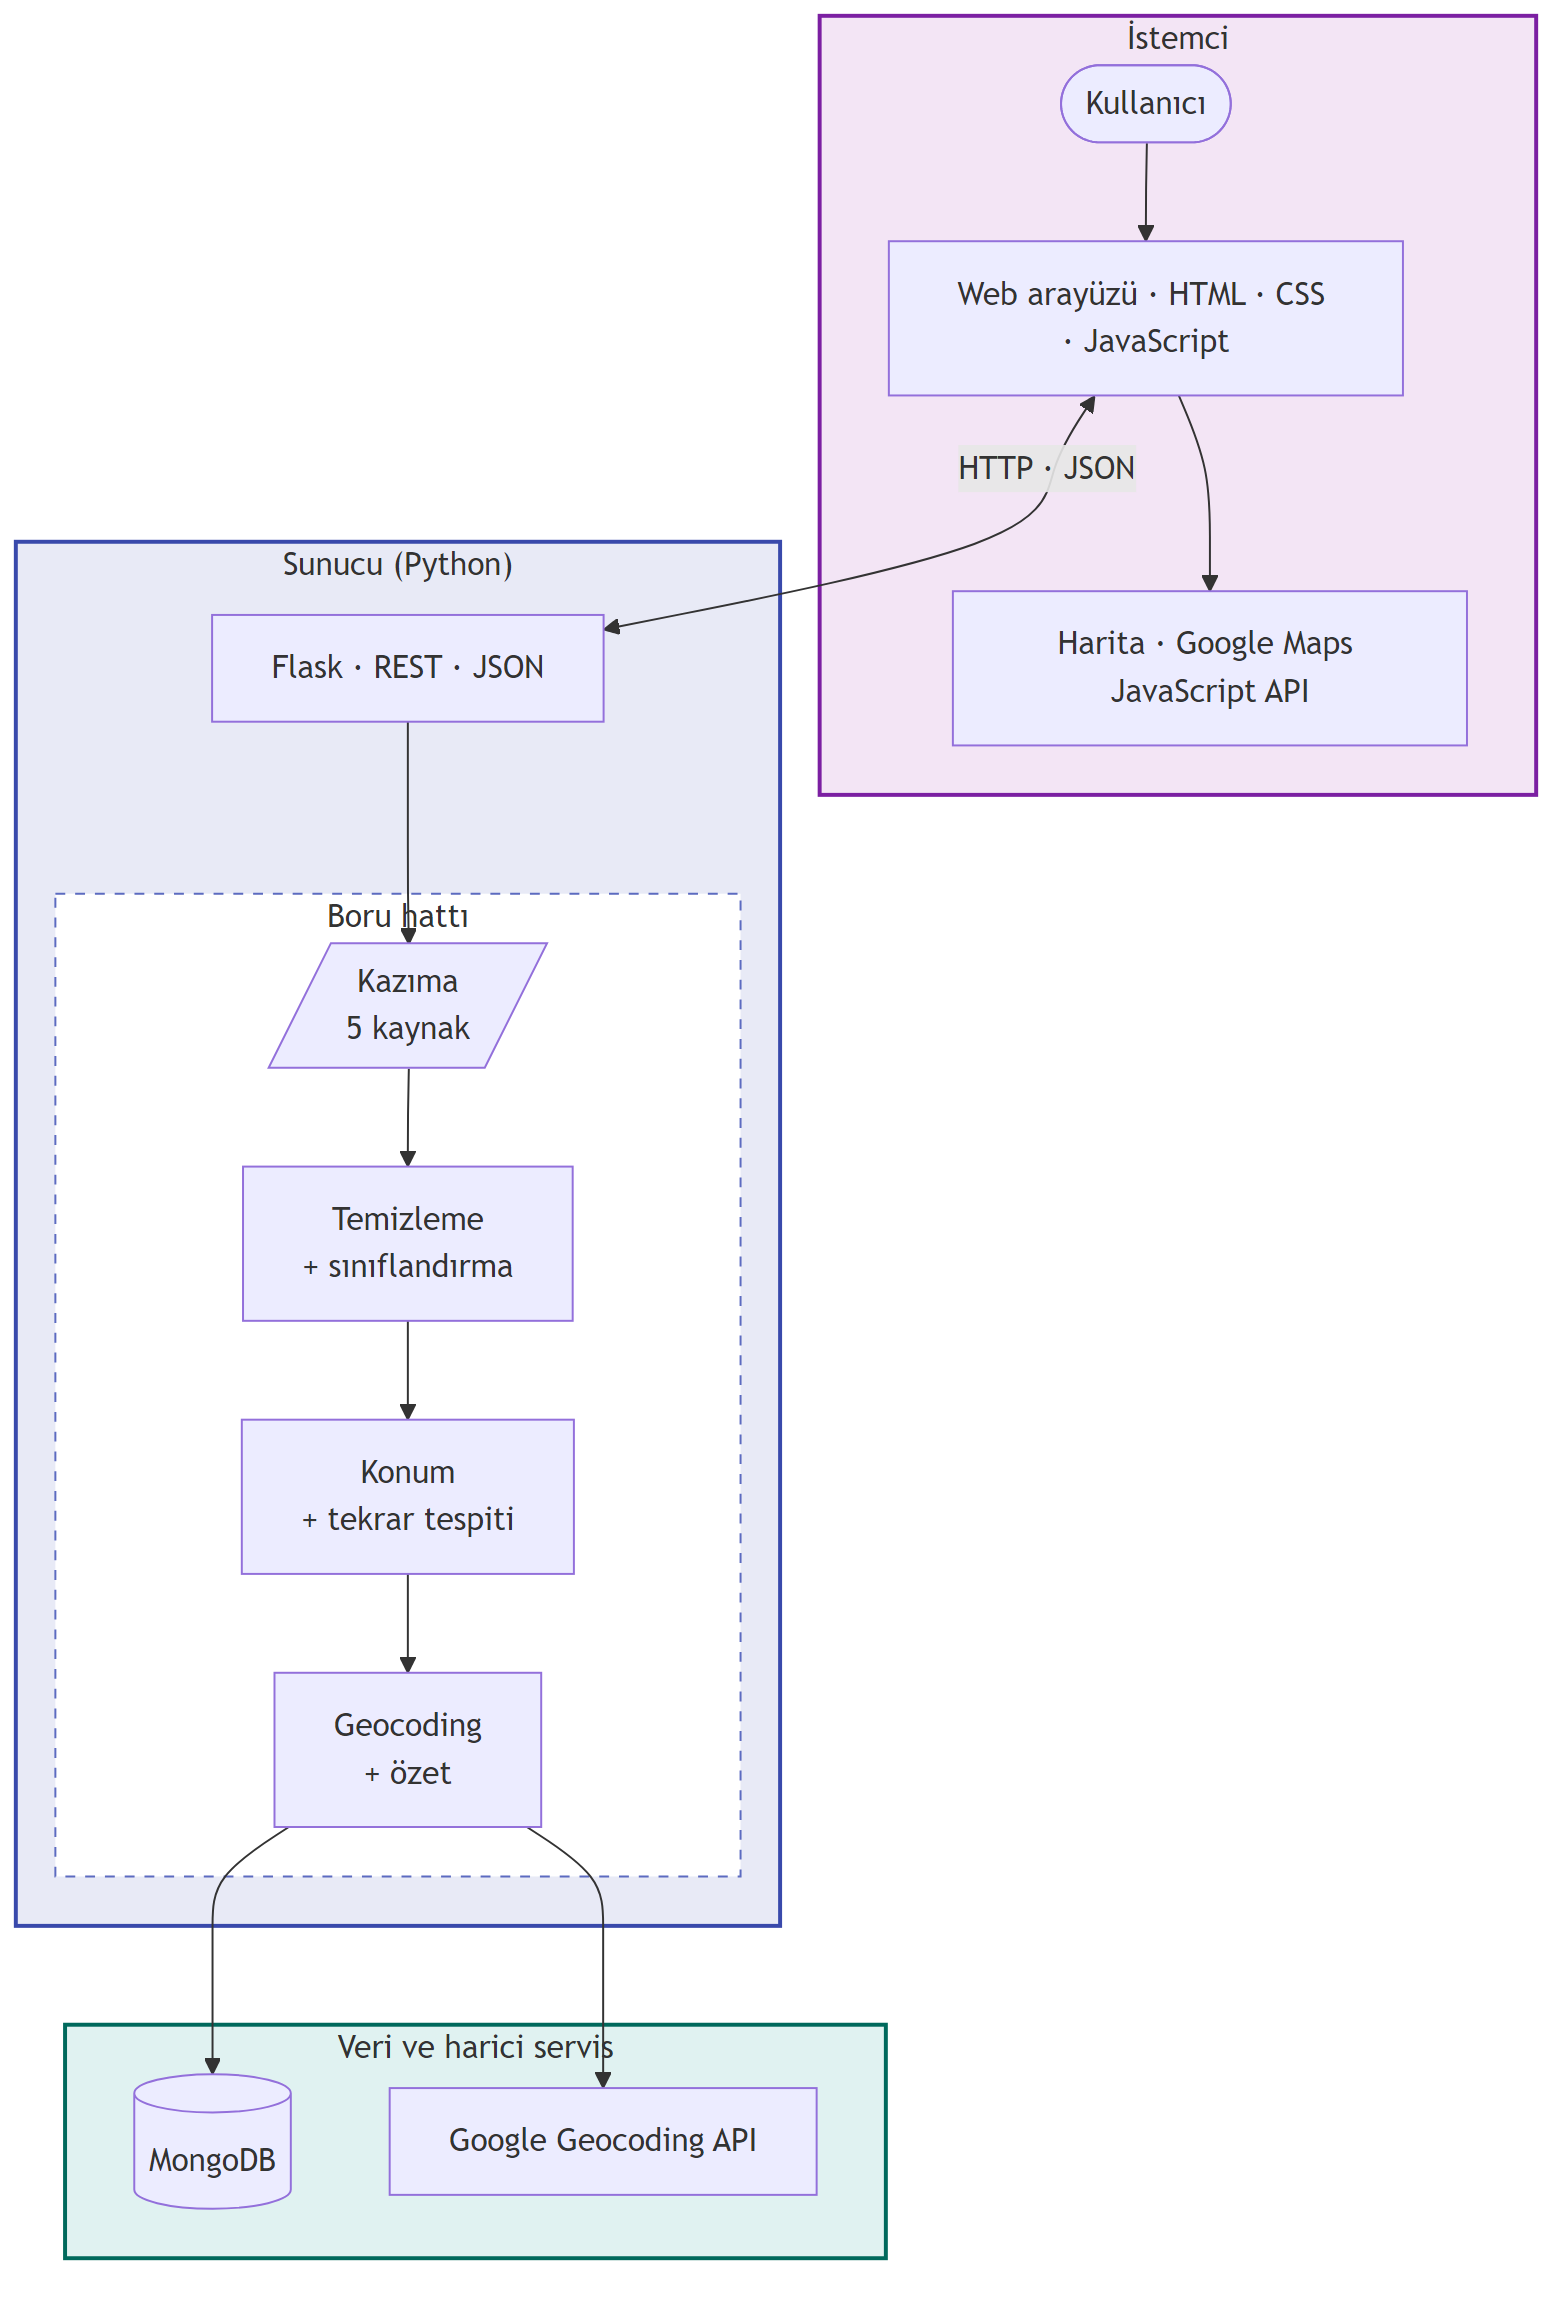
\includegraphics[width=0.96\textwidth]{resim/mimari_mermaid.pdf}%
}{%
  \IfFileExists{resim/mimari_mermaid.png}{%
    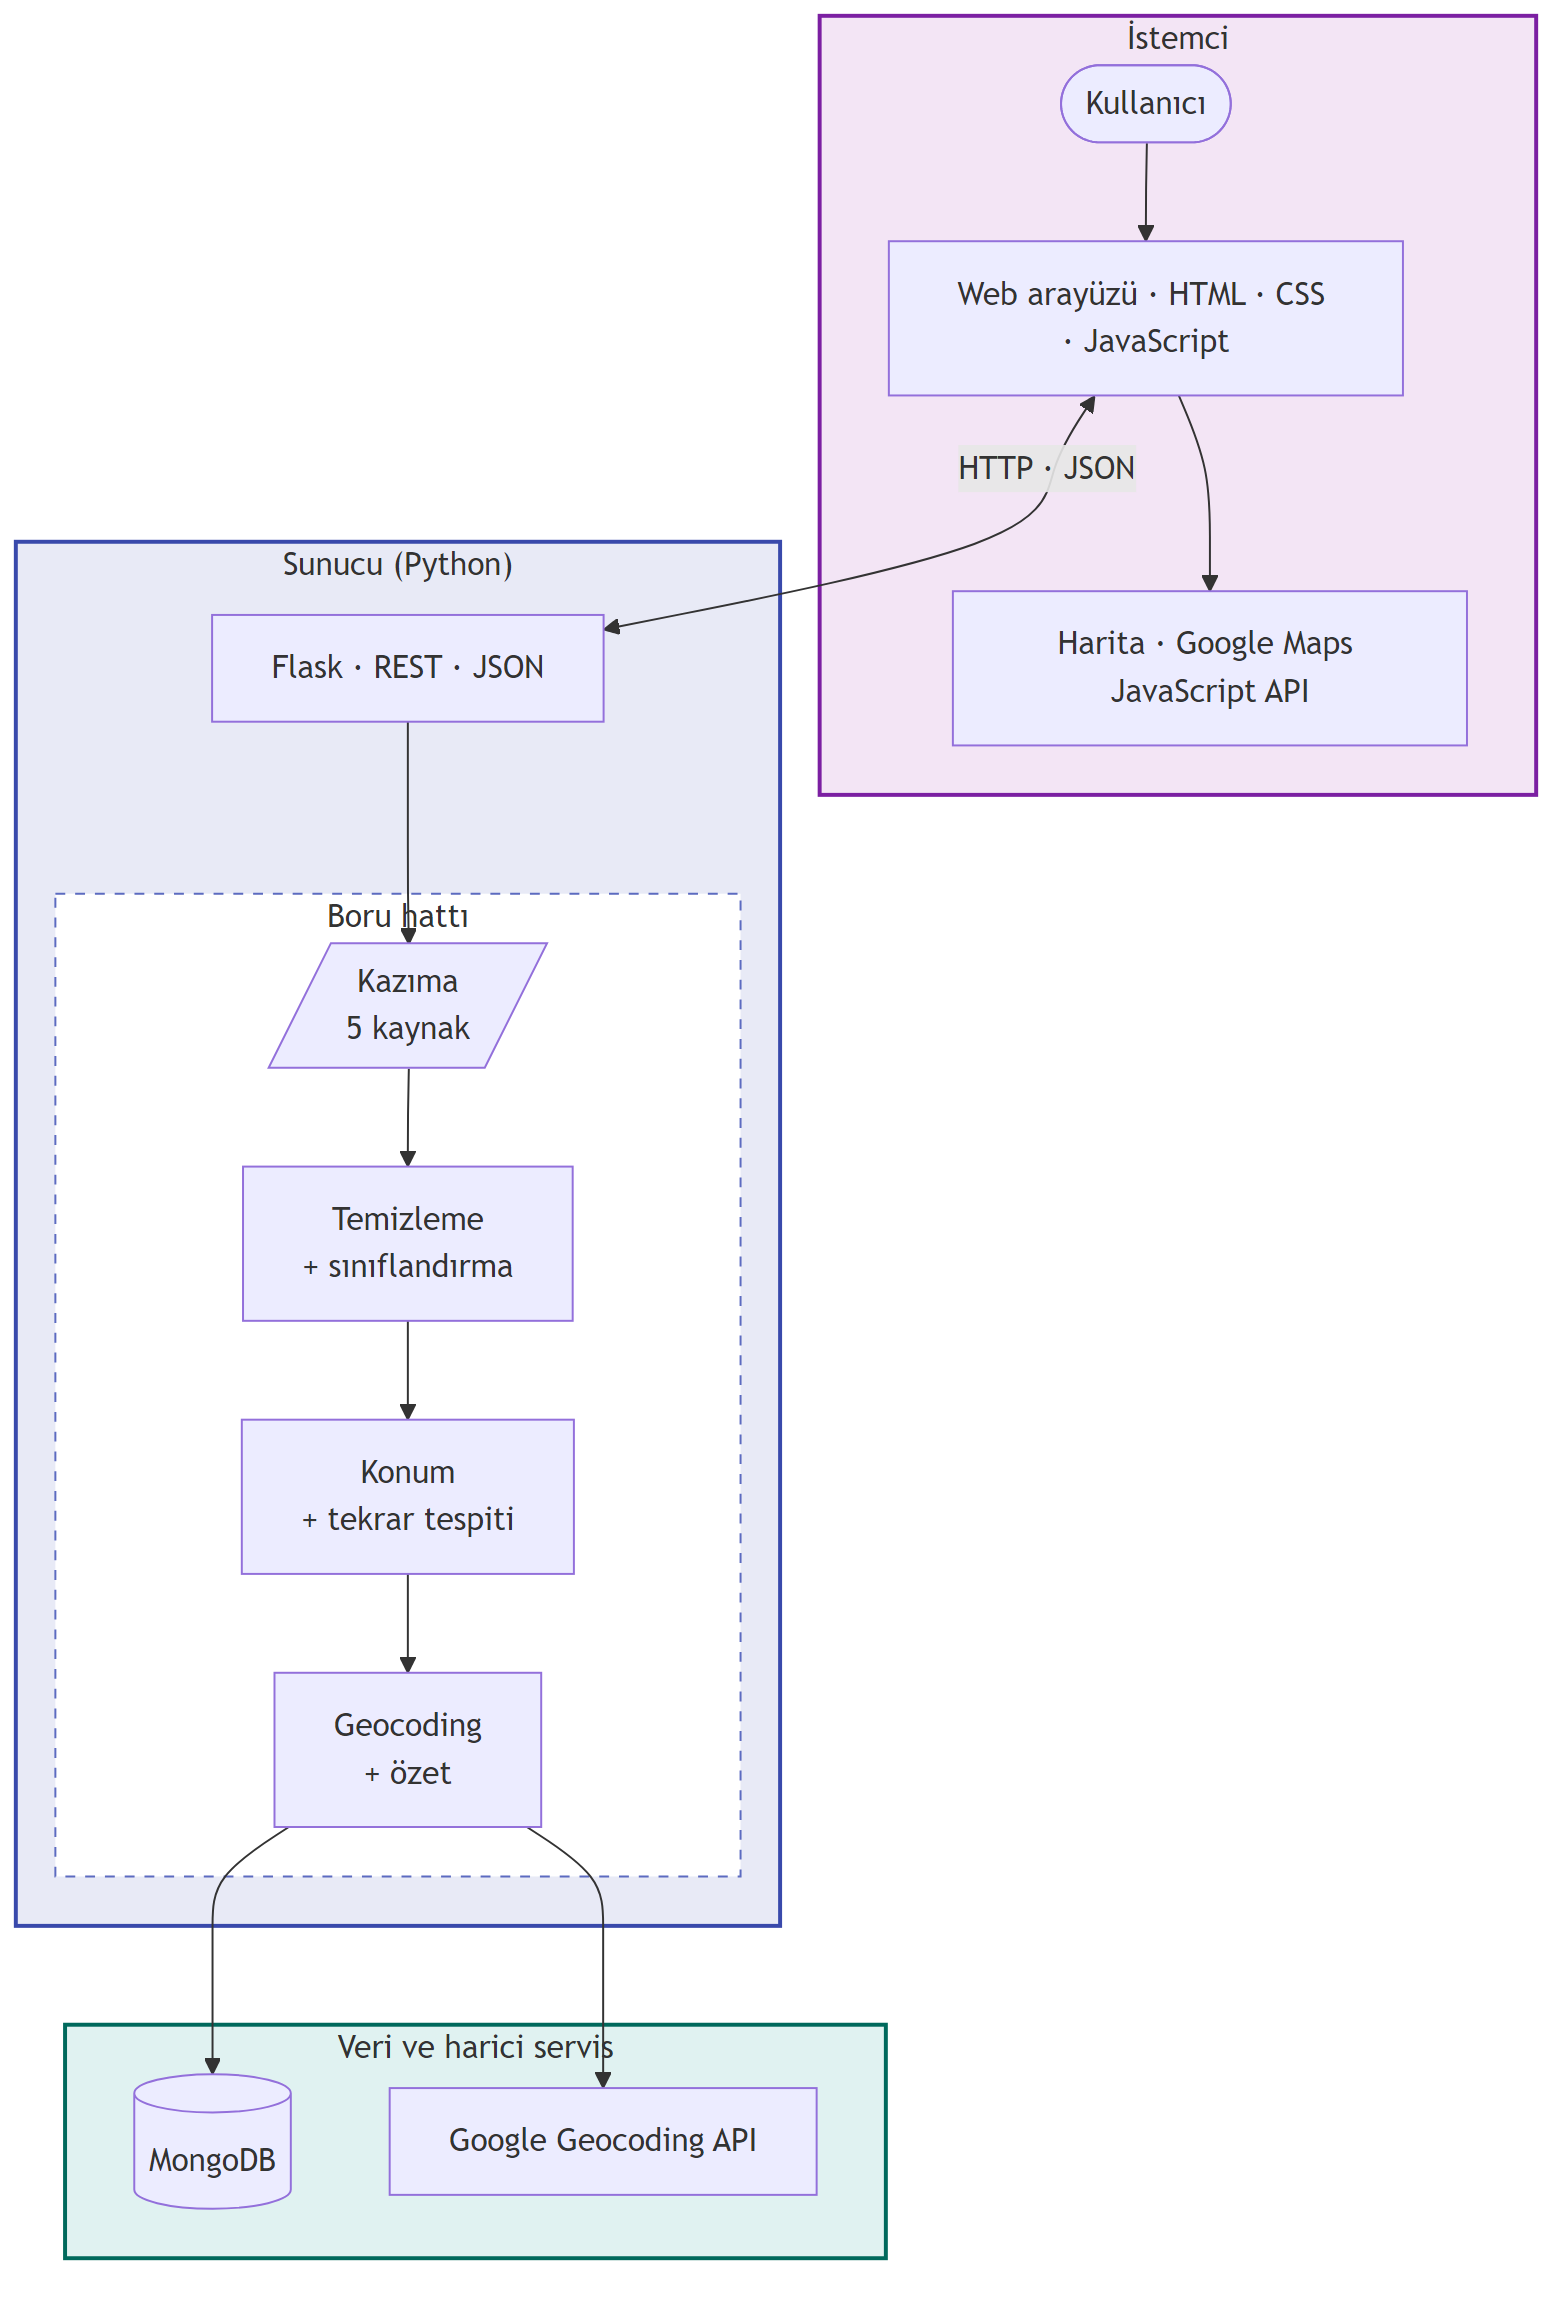
\includegraphics[width=0.96\textwidth]{resim/mimari_mermaid.png}%
  }{%
\resizebox{0.96\textwidth}{!}{%
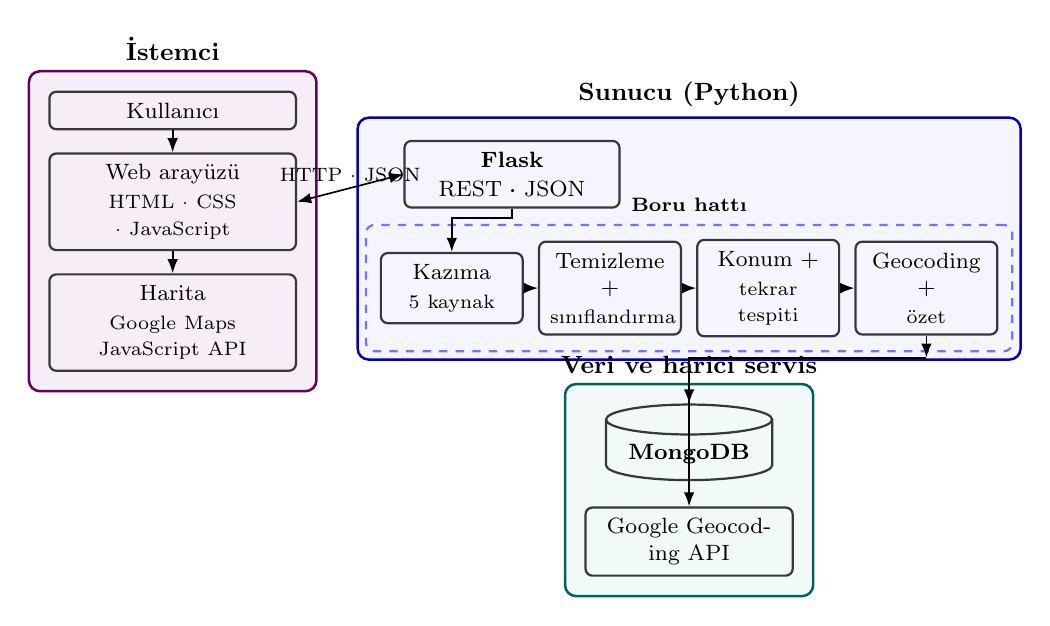
\begin{tikzpicture}[
  font=\footnotesize,
  box/.style={rectangle, rounded corners=2.5pt, draw=black!78, thick, align=center, inner sep=4pt},
  cyl/.style={cylinder, shape border rotate=90, aspect=0.18, draw=black!78, thick, align=center, inner sep=3pt, minimum height=0.62cm},
  arr/.style={-{Latex[length=1.8mm]}, semithick},
  darr/.style={{Latex[length=1.8mm]}-{Latex[length=1.8mm]}, semithick}
]
% --- İstemci ---
\node[box, text width=2.85cm] (U) {Kullanıcı};
\node[box, text width=2.85cm, below=0.28cm of U] (FE) {Web arayüzü\\[1pt]{\scriptsize HTML · CSS · JavaScript}};
\node[box, text width=2.85cm, below=0.28cm of FE] (MAP) {Harita\\[1pt]{\scriptsize Google Maps JavaScript API}};
\begin{scope}[on background layer]
  \node[draw=violet!75!black, line width=0.9pt, fill=violet!7, rounded corners=4pt, inner sep=7pt,
        fit=(U)(FE)(MAP), label={[font=\small\bfseries]above:İstemci}] {};
\end{scope}
% --- Sunucu ---
\node[box, text width=2.45cm, right=1.35cm of FE.east, anchor=west, yshift=0.35cm] (API) {\textbf{Flask}\\[1pt]REST · JSON};
\node[box, text width=1.52cm, below left=0.55cm and -0.15cm of API.south] (S1) {Kazıma\\[1pt]{\scriptsize 5 kaynak}};
\node[box, text width=1.52cm, right=0.18cm of S1] (S2) {Temizleme +\\[1pt]{\scriptsize sınıflandırma}};
\node[box, text width=1.52cm, right=0.18cm of S2] (S3) {Konum +\\[1pt]{\scriptsize tekrar tespiti}};
\node[box, text width=1.52cm, right=0.18cm of S3] (S4) {Geocoding +\\[1pt]{\scriptsize özet}};
\begin{scope}[on background layer]
  \node[draw=blue!68!black, line width=0.9pt, fill=blue!4, rounded corners=4pt, inner sep=8pt,
        fit=(API)(S1)(S2)(S3)(S4), label={[font=\small\bfseries]above:Sunucu (Python)}] {};
  \node[draw=blue!55, dashed, thick, rounded corners=3pt, inner sep=5pt,
        fit=(S1)(S2)(S3)(S4), label={[font=\scriptsize\bfseries,yshift=1pt]above:Boru hattı}] {};
\end{scope}
% --- Veri / harici ---
\node[cyl, text width=1.9cm, below=0.85cm of $(S2.south)!0.5!(S3.south)$, anchor=north] (DB) {\textbf{MongoDB}};
\node[box, text width=2.35cm, below=0.32cm of DB] (GEO) {Google Geocoding API};
\begin{scope}[on background layer]
  \node[draw=teal!75!black, line width=0.9pt, fill=teal!5, rounded corners=4pt, inner sep=7pt,
        fit=(DB)(GEO), label={[font=\small\bfseries]above:Veri ve harici servis}] {};
\end{scope}
% --- Oklar ---
\draw[arr] (U) -- (FE);
\draw[arr] (FE) -- (MAP);
\draw[darr] (FE.east) -- node[above, font=\scriptsize, inner sep=2pt] {HTTP · JSON} (API.west);
\draw[arr] (API.south) -- ++(0,-0.12) -| (S1.north);
\draw[arr] (S1) -- (S2);
\draw[arr] (S2) -- (S3);
\draw[arr] (S3) -- (S4);
\coordinate (Y) at ($(S4.south)+(0,-0.28)$);
\draw[arr] (S4.south) -- (Y);
\draw[arr] (Y) -| (DB.north);
\draw[arr] (Y) -| (GEO.north);
\end{tikzpicture}%
}%
  }%
}%
\caption{Sistemin yüksek seviye veri akışı ve bileşenleri. Aynı yapı \texttt{mermaid\_mimari.mmd} ile Mermaid olarak da tanımlanmıştır; istenirse \texttt{mmdc} ile PNG/PDF üretilip \texttt{resim/} altına konularak bu şeklin yerine konulabilir.}
\label{fig:arch}
\end{figure*}

\section{Yöntem}

\subsection{Yazılım Yığını}
Tablo~\ref{tab:stack} özet bileşenleri listeler. Sunucu tarafı Python~3 ile yazılmıştır; istemci saf HTML/CSS/JavaScript ve Google Maps JavaScript API kullanır.

\begin{table}[!t]
\caption{Kullanılan ana teknolojiler.}
\label{tab:stack}
\centering
\begin{tabular}{@{}ll@{}}
\toprule
Katman & Bileşen \\
\midrule
API & Flask, CORS, JSON \\
Veri & MongoDB (haberler, önbellek) \\
Kazıma & requests, BeautifulSoup, cloudscraper \\
Gömme & sentence-transformers (paraphrase-multilingual) \\
Harita & Google Maps Geocoding + JS API \\
\bottomrule
\end{tabular}
\end{table}

\subsection{Sınıflandırma}
Önceden tanımlı altı zorunlu kategori (ör.\ trafik kazası, yangın, elektrik kesintisi, hırsızlık, suç/cinayet, kültürel etkinlik) için başlık ve gövdede anahtar kelime eşleşmeleri ağırlıklı toplanır. Her eşleşme, kelimenin haber dilindeki güvenilirliğine göre farklı ağırlık alabilir; örneğin genel fiiller düşük, türü doğrudan çağrıştıran isimler yüksek ağırlıklıdır. URL yolu ve metin bağlamı için ceza ve güçlendirme kuralları uygulanır: finans veya borsa içeriklerinde kültürel etkinlik skoru baskılanır; su kesintisi ifadeleri elektrik kesintisi ile karıştırılmaması için cezalandırılır; meteoroloji, sinema veya sendika gündemi gibi bağlamlarda hırsızlık veya suç skorları düşürülür.

Skorların mutlak eşiği, yalnızca anahtar kelime/kural sinyali yeterince güçlü olduğunda sınıflandırmaya izin verecek biçimde ayarlanmıştır; eşik altında kalan haberler veri tabanına yazılmaz (gürültü azaltma). İsteğe bağlı olarak, her kategori için önceden tanımlı kısa Türkçe çapa metinleriyle cümle gömme benzerliği ek puan olarak eklenebilir; ancak bu katman tüm kategorilere eşzamanlı katkı verdiğinden yüksek ağırlıkta yanlış pozitif riski doğurabilir. Uygulamada bu ağırlık genellikle sıfır (kapalı) tutulur ve yalnızca anahtar kelime tabanlı skor eşiği geçildikten sonra etkinleştirilmesi tercih edilir. Eşit skor durumunda kategori öncelik sırası (ör.\ trafik ve yangın gibi acil olaylar önce) ile tek bir etiket seçilir. Tablo~\ref{tab:cat} örnek kelime ailelerini özetler (gerçek uygulamada liste çok daha geniştir).

\begin{table}[!t]
\caption{Örnek kategori ipuçları (özet).}
\label{tab:cat}
\centering
\footnotesize
\begin{tabular}{@{}p{0.35\columnwidth}p{0.55\columnwidth}@{}}
\toprule
Kategori & Örnek tetikleyiciler \\
\midrule
Trafik & kaza, çarpma, yol kapalı, TEM, D-100 \\
Yangın & duman, itfaiye, alevlendi \\
Elektrik & kesinti, SEDAŞ, trafo \\
Hırsızlık & hırsızlık, soygun, hırsız \\
Suç & cinayet, gözaltı, operasyon \\
Kültür & konser, sergi, festival \\
\bottomrule
\end{tabular}
\end{table}

\subsection{Tekrar Tespiti ve Birleştirme}
Paraphrase çok dilli MiniLM ailesinden bir model ile haber metninden gömme vektörü üretilir. Veri tabanında tutulan vektörlerle kosinüs benzerliği hesaplanır; önceden seçilen eşik üzerinde eşleşme varsa yeni URL mevcut kayıt altında \texttt{sources} listesine eklenir, böylece haritada tek pin altında çoklu kaynak gösterimi mümkün olur. Aynı kategorideki haberler için, başlık/metin farklı yazılmış ajans metinlerini yakalamak amacıyla biraz daha düşük bir eşik kullanılabilir; farklı kategorilerde ise birleştirme daha temkinli tutulur. Tüm kaynaklar tarandıktan sonra, aynı gün ve kategori için ikinci bir birleştirme geçişi (daha gevşek kosinüs ve başlık örtüşmesi) çoklu kaynak kartlarını iyileştirmeye yöneliktir. Boru hattı dışında, geçmişe dönük temizlik için ayrı bir birleştirme betiği de kullanılabilir; bu, model veya eşik değişimlerinden sonra tutarlılığı yeniden sağlamaya yarar.

\subsection{Özetleme}
Tam metin üzerinde cümle bölme, çok kısa veya yinelenen cümlelerin elenmesi ve gürültü filtrelemesi yapılır. Ardından başlığın gömme vektörü ile her cümlenin vektörü karşılaştırılır; başlığa anlamsal olarak yakın ve metinde erken bölgede yer alan cümleler önceliklendirilir. Seçilen birkaç cümle birleştirilerek kullanıcı arayüzünde gösterilecek özet oluşturulur. Bu yöntem üretken özetlemeye göre daha ucuz ve deterministiktir; cümleler kaynak metinden birebir alındığı için halüsinasyon riski düşüktür.

\subsection{Konum ve Geocoding}
Konum çıkarıcı, metinde geçen ilçe adları, bilinen yer isimleri ve URL parçalarından aday dizeler üretir. Adaylar öncelik sırasıyla Geocoding API'ye gönderilir; başarılı sonuç enlem/boylam ve standartlaştırılmış adres metni ile kayda yazılır. Aynı sorgu daha önce yapıldıysa \texttt{geocoding\_cache} koleksiyonundan okunur. Zincirde denenecek aday sayısı sınırlı tutulur. Yapılandırmaya bağlı olarak, tüm adaylar başarısız olduğunda kayıt İzmit merkezine yakın bir genel koordinata düşürülebilir; bu, haritada pin görünürlüğünü garanti eder fakat ``genel konum'' olarak işaretlenmeli ve otomatik adres doğruluğu açısından dikkatle yorumlanmalıdır. Aksi durumda haber listede kalırken haritada işaretsiz olabilir.

\subsection{REST Arayüzü ve Eşzamanlılık}
Örnek uç noktalar: sağlık kontrolü (\texttt{/api/health}), filtre parametreleriyle haber listesi (\texttt{/api/news}), kategori ve ilçe listeleri, istatistik (\texttt{/api/stats}; yanıtta \texttt{by\_source} ve \texttt{by\_category} alanları), yapılandırma (\texttt{/api/config}) ve yapılandırılabilir tarama tetikleyicisi (\texttt{/api/scrape}). Uzun süren tarama işlemi arka planda iş parçacığında yürütülür; istemci yanıtı hemen döner ve durum bayrakları ile ilerleme izlenir. Önceki sürümlerde iş parçacığı sonlandıktan sonra ``çalışıyor'' bayrağının takılı kalması HTTP~409 çakışmasına yol açabiliyordu; güncel tasarımda iş parçacığı nesnesi üzerinde canlılık kontrolü ile bayrak tutarlı hale getirilmiştir.

\subsection{Ön Uç Davranışı}
Statik dosyalar ayrı bir HTTP sunucusu üzerinden sunulabilir; tarayıcı API taban URL'sini yapılandırarak Flask ile konuşur. Harita yüklemesi için API anahtarı gereklidir. Kaynak listesinde aynı sitenin birden fazla kez görünmesi kullanıcıyı yanıltabileceğinden, istemci tarafında URL ve görünen kaynak adına göre tekilleştirme uygulanmıştır. Üst bantta kaynak sayımları, hangi sitelerin son taramada veri ürettiğini hızlıca gösterir.

\section{Deneysel Gözlemler ve Tartışma}
Gerçek ortamda kaynak başına çekilen haber sayısı ağ gecikmesi, site şablon değişiklikleri ve erişim politikalarına bağlıdır. Dört sitenin düzenli veri ürettiği, bir sitenin sürekli HTTP~403 döndürdüğü gözlemlenmiştir; bu durum kazıyıcı mantık hatasından çok Cloudflare veya benzeri koruma katmanlarıyla uyumludur. \texttt{cloudscraper} gibi araçlar bazı senaryolarda yardımcı olur ancak tüm korumaları aşmayı garanti etmez; kalıcı çözüm genellikle resmi API, iş birliği veya tarayıcı otomasyonu ve IP/itibar yönetimi gibi daha ağır yatırımlar gerektirir.

Sınıflandırma kural seti genişletildikçe yanlış pozitifler (ör.\ altyapı veya meteoroloji haberinin trafik veya hırsızlık sanılması) azaltılabilir. Bununla birlikte kural tabanlı sistemlerde sınır örnekler her zaman kalır; özellikle çok olaylı başlıklarda tek bir etiket zorlanması hatalı özet oluşturabilir. Gömme tabanlı özet, üretken modellere göre daha düşük maliyetlidir fakat yeni ifadeler üretmez; başlıkla zayıf ilişkili cümleler seçilirse özet yine yetersiz kalabilir.

\subsection{Doğrulama ve Kalite Güvencesi}
Kod tabanında kazıyıcı çıktıları, site erişilebilirliği ve coğrafi kodlama için yardımcı doğrulama betikleri bulunmaktadır; sınıflandırıcı ise geliştirme sırasında tipik yanlış pozitif örnekleri (altyapı, afet farkındalığı, otoyol kazası vb.) hedefleyen kural güncellemeleri ile gözle kontrol edilmiştir. Otomatik testler UTF-8 ve ortam faktörlerine duyarlı olabileceğinden, sürekli entegrasyon ortamında aynı kod sayfası ile çalıştırılması önerilir. Tekrar tespiti için eşik değeri, hem fazla birleştirmeyi hem de kaçırılan duplicateleri dengeleyecek şekilde ayarlanmalıdır.

\subsection{Performans ve Ölçeklenebilirlik}
Gömme modeli ilk yüklemede bellek ve süre maliyeti oluşturur; boru hattı boyunca vektörler bir kez hesaplanıp saklandığında sonraki sorgular hızlanır. MongoDB indeksleri, URL benzersizliği ve tarih aralığı filtrelerinde gecikmeyi düşürür. Geocoding önbelleği, tekrarlayan ilçe ve mahalle adlarında API maliyetini belirgin biçimde azaltır. Ön uçta kaynak istatistik çubuğu, kullanıcıya veri tazeliği hakkında hızlı geri bildirim sağlar.

\subsection{Kısıtlar}
\begin{itemize}
\item WAF/Cloudflare korumalı kaynaklar otomatik kazımayı engelleyebilir.
\item Kural tabanlı sınıflandırma, dil değişimi ve yeni argo için periyodik bakım ister.
\item Geocoding, belirsiz adreslerde yanlış veya eksik koordinat üretebilir; merkez düşümü etkinse haritada genel pin görünür ancak gerçek olay yeriyle örtüşmeyebilir.
\item Üretken özet veya çok modlu (görüntü) içerik işleme kapsam dışıdır.
\end{itemize}

\section{Gelecek Çalışmalar}
Öncelikli adımlar: (i) erişim engeli yaşayan kaynaklar için Playwright tabanlı tarayıcı otomasyonu ve sorumlu hız sınırlama, (ii) sınırlı etiketli veri ile hafif bir denetimli ince ayar veya çok sınıflı sınıflandırıcı, (iii) kullanıcı geri bildirimiyle kural ağırlıklarının güncellenmesi, (iv) özet kalitesi için isteğe bağlı küçük dil modeli veya çıkarımsal üretken özetleme. Ayrıca harita üzerinde yoğunluk ısı haritası ve zaman çizelgesi görünümü, kentsel olay analitiğine değer katabilir.

\section{Sonuç}
Çalışma, Kocaeli yerel haber ekosistemini tek bir harita ve API üzerinde birleştiren uçtan uca bir iskelet sunmaktadır. Modüler kazıyıcılar, kural tabanlı sınıflandırma, gömme ile tekrar yönetimi ve önbellekli geocoding birlikte düşünüldüğünde, benzer şehir ölçekli projeler için yeniden kullanılabilir bir şablon oluşturur. En büyük pratik engel, teknik boru hattından çok kaynak sitelerinin erişim politikalarıdır; bu nedenle operasyonel sürdürülebilirlik, yazılım kadar iletişim ve uyum süreçleriyle de ilgilidir.

% ---------- FIG_TEAM: Fotoğrafı buraya ekleyin ----------
% 1) Görseli şu klasörlerden birine koyun: rapor/ veya rapor/resim/
% 2) Aşağıdaki \includegraphics satırının başındaki % işaretini kaldırın.
% 3) Dosya adını kendi dosyanızla değiştirin (jpg, png, pdf olabilir).
% 4) İsterseniz width=0.85\columnwidth değerini büyütüp küçültün.
\begin{figure}[H] % [H] ile resmi tam oraya çiviliyoruz
    \centering
    \includegraphics[width=1.0\columnwidth]{project_image.jpg} 
    \caption{Kocaeli Haber Haritası - Genel Görünüm}
    \label{fig:harita_full}
\end{figure}

\section*{Teşekkür}
Bu rapor, ders kapsamındaki proje geliştirme sürecinin özetidir.

\begin{thebibliography}{00}
\bibitem{scraping}
R. Mitchell, \textit{Web Scraping with Python}, 2nd ed. O'Reilly Media, 2018.

\bibitem{reimers2019}
N. Reimers and I. Gurevych, ``Sentence-BERT: Sentence embeddings using Siamese BERT-networks,'' in \textit{Proc. EMNLP-IJCNLP}, 2019, pp. 3982--3992.

\bibitem{googlegeo}
Google, ``Geocoding API Overview,'' Google Maps Platform documentation. Erişim: \url{https://developers.google.com/maps/documentation/geocoding}

\bibitem{flask}
Pallets Projects, ``Flask Web Framework,'' \url{https://flask.palletsprojects.com/}

\bibitem{mongo}
MongoDB Inc., ``MongoDB Documentation,'' \url{https://www.mongodb.com/docs/}
\end{thebibliography}

\end{document}
